\documentclass{beamer}
\usepackage{amsthm,amsmath,amssymb,amsfonts,amscd}
\usepackage{graphicx}
\usepackage{subcaption}
\usepackage{enumerate}
\usepackage[all]{xy}
\usepackage{booktabs}
\usepackage{wrapfig}
\usepackage{float}
\usepackage[english]{babel}
\usepackage[scr=boondoxo]{mathalfa}
% \usepackage[nottoc]{tocbibind}
\usepackage[justification=centering]{caption}
\usepackage{mathtools}
\usepackage{setspace}
\usepackage{stmaryrd}
\usepackage{multicol}
\usepackage{xcolor}
\usepackage{bbm}
\usepackage[utf8]{inputenc}
\usepackage[round]{natbib}  
% \bibliographystyle{plainnat}

\usepackage{tikz}
\usetikzlibrary{decorations.pathreplacing,calligraphy}
\usetikzlibrary{positioning}
\usetikzlibrary{shapes}
\usetikzlibrary{arrows.meta}
\usetikzlibrary{tikzmark}


\usepackage[final]{pdfpages}
\usepackage{relsize}

\mode<presentation>
{
  \usetheme{Boadilla}  
  \usecolortheme{beaver}
  \setbeamercolor{author in head/foot}{fg=white,bg=mygreen}
  \setbeamercolor{title in head/foot}{fg=mygreen,bg=mygreengray}
  \setbeamercolor{date in head/foot}{fg=mygreen,bg=white}
  \setbeamercolor{page number in head/foot}{fg=white,bg=mygreen}
  
  \usefonttheme{default}
  \setbeamercolor{title}{fg=mygreen}
  \setbeamercolor{frametitle}{fg=mygreen}
  \setbeamertemplate{navigation symbols}{}
  \setbeamertemplate{caption}[numbered]
  \setbeamercolor{section number projected}{bg=mywhite,fg=mygreen}
  \setbeamercolor{subsection number projected}{bg=mygreen,fg=mygreen}
  \setbeamercolor{subsubsection number projected}{bg=mywhite,fg=mygreen}
  \setbeamertemplate{itemize item}{\color{mygreen}$\star$}
  \setbeamertemplate{itemize subitem}{\color{mygreen}$\triangleright$}
  \setbeamertemplate{itemize subsubitem}{\color{mygreen}$\triangleright$}
  % Customize enumerate items
  \setbeamertemplate{enumerate items}[default]
  \setbeamercolor{enumerate item}{fg=mygreen,bg=mygray}
}

\definecolor{mygray}{HTML}{7C6C6C}
\definecolor{mygreen}{HTML}{53b679}
\definecolor{myred}{HTML}{BB0C0C}
\definecolor{mypurple}{HTML}{800080}
\definecolor{mywhite}{HTML}{DDDDDD}
\definecolor{mygreengray}{HTML}{e1e8e3}

\newcommand{\pmm}{PM$_{2.5}$}
\newcommand{\oo}{O$_{3}$}

\newcommand{\R}{\ensuremath{\mathbb{R}}}
\renewcommand{\deg}{$^\circ$}



%----------------------------------------------------------------------------------------
%	TITLE PAGE
%----------------------------------------------------------------------------------------

\title[Air pollution health damages]{Methods for the assessment of air pollution health damages}

\author[Clàudia Rodés Bachs - BC3]{Clàudia Rodés Bachs\\[3mm]Basque Centre for Climate Change}
\date{February 13, 2024}
\titlegraphic{\includegraphics[width=3cm]{extraFigs/BC3_logo.png}}

% logo
\newcommand\AtPagemyUpperLeft[1]{\AtPageLowerLeft{%
\put(\LenToUnit{0.85\paperwidth},\LenToUnit{0.895\paperheight}){#1}}}
\AddToShipoutPictureFG{
  \AtPagemyUpperLeft{{\includegraphics[height=1cm,keepaspectratio]{extraFigs/BC3_logo.png}}}
}


\begin{document}

\begin{frame}
\titlepage 
\begin{tikzpicture}[remember picture, overlay]
  \fill[white] ([xshift=6.5cm, yshift=7.5cm] current page.center) rectangle ++(-2cm,-2cm);
\end{tikzpicture}
\end{frame}

\begin{frame}
\frametitle{Outline}
\tableofcontents 
\end{frame}

%--------------------------------
%	PRESENTATION SLIDES
%--------------------------------

\section{Scientific evidence: Why does climate change affect our health and economy?} 
\begin{frame}
\begin{center}
\Huge Scientific evidence: Why does \textcolor{mypurple}{climate change} affect our \textcolor{mygreen}{health} and \textcolor{mygreen}{economy}?
\end{center}
\end{frame}
%------------------------------------------------

\begin{frame}
\frametitle{Outdoor air pollution in numbers}
According to IHME database (\cite{ihme_gbd_2019}), in 2019...\vspace{1cm}
\begin{center}
    4.505 (95\% CI 3.625-5.364) million deaths\\\vspace{1cm}
    124.21 (95\% CI 398.89-147.63) disability-adjusted life years (DALYs)\\
\end{center}
\end{frame}


\begin{frame}
\frametitle{Pollutants origin}
\centering
    \begin{tikzpicture}[
    roundnode1/.style={circle, draw=green!60, fill=green!5, very thick, minimum size=15mm},
    ]
    %Nodes
    \onslide<1-8>{\node[roundnode1] (pmm) at (2,1) {\pmm};}
    \onslide<1-8>{\node[roundnode1] (oo) at (7,1) {\oo};}
    \onslide<2-8>{\node[draw=white, align = center] (ff) at (4.5,-2) {\includegraphics[width=4cm]{"Images_intro/fossil_fuel.png"}};}
    \onslide<3-8>{\node[cloud, draw, text width=1.5cm, align = center] (ghg) at (8,-4) {GHG emissions};}
    \onslide<4-8>{\node[draw=white] (earth) at (11,-1) {\includegraphics[width=3.2cm]{"Images_intro/earth.png"}};}
    
    \onslide<2-8>{\draw[line width=6pt,purple,-{Triangle[width=1.8*6pt,length=0.8*6pt,purple]}](ff) to [out=135,in=300] (pmm);}
    \onslide<2-8>{\draw[line width=6pt,purple,-{Triangle[width=1.8*6pt,length=0.8*6pt,purple]}](ff) to [out=45,in=225] (oo);}
    \onslide<3-8>{\draw[line width=6pt,purple,-{Triangle[width=1.8*6pt,length=0.8*6pt,purple]}](ff) to [out=280,in=200] (ghg);}
    \onslide<4-8>{\draw[line width=6pt,purple,-{Triangle[width=1.8*6pt,length=0.8*6pt,purple]}](ghg) to [out=15,in=260] (earth);}
    
    % decrease arrow
    \onslide<5-8>{\draw[line width=6pt,green,-{Triangle[width=1.8*6pt,length=0.8*6pt,green]}](9.15,0) to (9.15,-2);}
    \onslide<6-8>{\draw[line width=6pt,green,-{Triangle[width=1.8*6pt,length=0.8*6pt,green]}](6.5,-3) to (6.5,-5);}
    \onslide<7-8>{\draw[line width=6pt,green,-{Triangle[width=1.8*6pt,length=0.8*6pt,green]}](2.45,-1) to (2.45,-3);}
    \onslide<8-8>{\draw[line width=6pt,green,-{Triangle[width=1.8*6pt,length=0.8*6pt,green]}](1,1.5) to (1,0.5);}
    \onslide<8-8>{\draw[line width=6pt,green,-{Triangle[width=1.8*6pt,length=0.8*6pt,green]}](6,1.5) to (6,0.5);}
\end{tikzpicture}
\end{frame}

\begin{frame}
\frametitle{\pmm\ map}
\centering
\href{https://www.iqair.com/earth}{\textcolor{blue}{\pmm\ map}}
\href{https://www.iqair.com/earth}{(\textcolor{blue}{https://www.iqair.com/earth})}
\end{frame}

\begin{frame}
\frametitle{Health impact of \pmm}
\begin{figure}
    \includegraphics[width = 0.8\linewidth]{Images_intro/pm_impacts.png}
\end{figure}
\vfill \hfill \tiny{\cite{basith_impact_2022}}
\end{frame}

\begin{frame}
\frametitle{Health impacts of \pmm\ \& \oo}
\centering
\href{https://vizhub.healthdata.org/gbd-compare/}{\textcolor{blue}{IHME database}}
\href{https://vizhub.healthdata.org/gbd-compare/}{(\textcolor{blue}{\texttt{https://vizhub.healthdata.org/gbd-compare/}})}
\end{frame}


\begin{frame}
\frametitle{Air pollution health and economic implications}
\begin{itemize}
    \setlength\itemsep{0.3cm}
    \item Premature deaths
    \item Years of Life Lost (YLLs)
    \item Disability Adjusted Life Years (DALYs)
    \item ...
\end{itemize}
\vspace{0.35cm}
\begin{center}
\pause\text{\Large$ \Downarrow $}
\end{center}
\vspace{0.35cm}
\begin{itemize}
    \setlength\itemsep{0.3cm}
    \item Economy growth
    \item Human Capital Lost (HCL)
    \item Value of Statistical Life (VSL)
    \item ...
\end{itemize}
\end{frame}



% %------------------------------------------------

\section{Brief overview of climate policies} 
\begin{frame}
\begin{center}
\Huge Brief overview of \textcolor{mygreen}{climate policies}
\end{center}
\end{frame}
%------------------------------------------------

\begin{frame}
\frametitle{Climate policies overview}
\begin{alertblock}{Paris Agreement main objective (2015) \textbf{(Current Policies (CP))}}
    To limit warming well below 2\deg C and pursue limiting it to 1.5\deg C    
\end{alertblock}
\vspace{1cm}
\onslide<2>{
\begin{alertblock}{Post-Glasglow Contributions (2021) \textbf{(Nationally Determined Contributions (NDC))}}
    To revisit and strengthen the countries 2030 emissions reduction targets
\end{alertblock}
 %In the two years preceding the negotiations in Glasgow, approximately 150 countries 
 % submitted a new or updated nationally determined contribution (NDC), most of which 
 % contained emissions reduction targets to be achieved by 2030
}
\end{frame}

\begin{frame}
    \frametitle{Climate policies pathways}

    \begin{columns}[T] 
        \begin{column}{0.66\textwidth} 
            \centering
            \includegraphics[width=\textwidth]{Images_intro/CP_NDC.png}
        \end{column}
        \begin{column}{0.33\textwidth}
            By 2030, 166623 (72789 - 260347 95\% CI) annual avoided premature deaths due to the CP, and 361744 (151698 - 571779 95\% CI) avoided premature deaths due to the NDC
            \\\vspace{0.25cm}
            \onslide<2>{To apply the NDC over the CP, avoids 195121 premature deaths}
        \end{column}
    \end{columns}
    \vfill\hfill\cite{sampedro_short-term_2023}
\end{frame}
        

\begin{frame}
    \frametitle{Climate policies pathways}
    \begin{table}[htb!]
    \centering
    \begin{tabular}{ccc}
    \toprule
    Temperature increase  & \qquad & Carbon budgets (GtCO$_2$) \\\hline
    Range around 1.5\deg C   & \qquad & 200, 300, 400, 500, 600, 700, 800, 900 \\
    Range around 1.5-2\deg C & \qquad & 1000, 1200, 1400, 1600, 1800, 2000 \\
    Higher budgets  & \qquad & 2500, 3000 \\
    \bottomrule 
    \end{tabular}
    \caption{Source: \citet{riahi_cost_2021}}
    \end{table}
\end{frame}

\begin{frame}
    \frametitle{Climate policies pathways}
    \centering
    \begin{tabular}{cc}
        \includegraphics[height=0.475\textwidth]{Images_intro/sketch_eoc.png}
        &\onslide<2>{
        \includegraphics[height=0.475\textwidth]{Images_intro/sketch_nz.png}}\\                                            
        Overshooting climate policy & \onslide<2>{Non-overshooting climate policy}\\
        \emph{end-of-century} & \onslide<2>{\emph{net-zero}}
    \end{tabular}
\end{frame}
    

% %------------------------------------------------

\section{How can we compute the air pollution damage?} 
\begin{frame}
\begin{center}
\Huge How can we compute the \textcolor{mypurple}{air pollution damage}?
\end{center}
\end{frame}
%------------------------------------------------

\begin{frame}
\frametitle{Computational Flow}
\vspace{-1.5cm}
\begin{figure}
    \centering
    \includegraphics[height=\textheight]{Images_flow/regions.png}
\end{figure}
\end{frame}


\begin{frame}
\frametitle{Computational Flow}
\begin{center}
\begin{tikzpicture}[trim left=(conc), trim right = (mort), node distance = 0.15cm]
    \onslide<1-5>{\node[draw,ellipse,text width=3cm,align=center] (eng) {\tiny{Detailed database}};}

    \onslide<2-8>{\node[draw=mypurple,rectangle,rounded corners, yshift = -1cm] (emi) [below left = of eng] {\includegraphics[width=2.7cm]{"Images_flow/plot_engage.png"}};}    
    \onslide<3-8>{\node[draw=mypurple,rectangle,rounded corners] (conc) [right = of emi] {\includegraphics[width=2.7cm]{"Images_flow/plot_conc.png"}};}    
    \onslide<4-8>{\node[draw=mypurple,rectangle,rounded corners] (mort) [right = of conc] {\includegraphics[width=2.7cm]{"Images_flow/plot_mort.png"}};}    
    \onslide<5-8>{\node[draw=mypurple,rectangle,rounded corners] (econ) [right = of mort] {\includegraphics[width=2.7cm]{"Images_flow/plot_econ.png"}};}
    
    % red frames
    \onslide<8-8>{\node[draw=red,rectangle,rounded corners,yshift = -0.5cm] (emiUncert) [below = of emi] {\includegraphics[width=2.7cm]{"Images_flow/plot_uncert_E.png"}};}    
    \onslide<8-8>{\node[draw=red,rectangle,rounded corners,yshift = -0.5cm] (concUncert) [below = of conc] {\includegraphics[width=2.7cm]{"Images_flow/plot_uncert_C.png"}};}    
    \onslide<8-8>{\node[draw=red,rectangle,rounded corners,yshift = -0.5cm] (mortUncert) [below = of mort] {\includegraphics[width=2.7cm]{"Images_flow/plot_uncert_M.png"}};}
    \onslide<8-8>{\node[draw=red,rectangle,rounded corners,yshift = -0.5cm] (econUncert) [below = of econ] {\includegraphics[width=2.7cm]{"Images_flow/plot_uncert_Econ.png"}};}

    \onslide<6-8>{\node[draw=red,ellipse,text width=3cm,align=center,text=red] (eng) {\tiny{Detailed database}};}
    \onslide<6-8>{\draw [->,red] (eng) to [out=180,in=130] node [text width=2.5cm,align=center,midway,above,red] {} (emi);}
    \onslide<6-8>{\draw [->,red] (emi) to [out=50,in=130] node [text width=2.5cm,align=center,midway,above,red] {\tiny{Chemical model}} (conc);}
    \onslide<6-8>{\draw [->,red] (conc) to [out=50,in=130] node [text width=2.5cm,align=center,midway,above,red] {\tiny{Impact functions}} (mort);}
    \onslide<6-8>{\draw [->,red] (mort) to [out=50,in=130] node [text width=2.5cm,align=center,midway,above,yshift=0.25cm] {\tiny{Econometric}} (econ);}
    \onslide<6-8>{\draw [->,red] (mort) to [out=50,in=130] node [text width=2.5cm,align=center,midway,above,xshift=0.25cm] {\tiny{equations}} (econ);}
    \onslide<6-8>{\draw [->,red] (1,-1.3) .. controls (2,-0.5) and (4,-0.5) .. (5,-1.3);}
  
    % Text
    \onslide<2-8>{\node (emiText) [above of=emi,text width=2cm,yshift=0.85cm,align=center,mypurple]{\tiny{Estimated emissions}};;}    
    \onslide<3-8>{\node (concText) [above of=conc,text width=3cm,yshift=0.85cm,align=center,mypurple]{\tiny{Computed concentrations}};;}    
    \onslide<4-8>{\node (mortText) [above of=mort,text width=2cm,yshift=0.85cm,align=center,mypurple]{\tiny{Health impact}};;}    
    \onslide<5-8>{\node (econText) [above of=econ,text width=2cm,yshift=0.85cm,align=center,mypurple]{\tiny{Economic impact}};;}

    % Arrows
    \onslide<2-6>{\draw [->,black] (eng) to [out=180,in=130] node [text width=2.5cm,align=center,midway,above] {} (emi);}

    \onslide<3-6>{\draw [->] (emi) to [out=50,in=130] node [text width=2.5cm,align=center,midway,above] {\tiny{Chemical model}} (conc);}
    \onslide<4-6>{\draw [->] (conc) to [out=50,in=130] node [text width=2cm,align=center,midway,above] {\tiny{Impact functions}} (mort);}    
    \onslide<5-6>{\draw [->] (mort) to [out=50,in=130] node [text width=2.5cm,align=center,midway,above,yshift=0.25cm] {\tiny{Econometric}} (econ);}
    \onslide<5-6>{\draw [->] (mort) to [out=50,in=130] node [text width=2.5cm,align=center,midway,above,xshift=0.25cm] {\tiny{equations}} (econ);}
    \onslide<5-6>{\draw [->] (1,-1.3) .. controls (2,-0.5) and (4,-0.5) .. (5,-1.3);}
    
    \onslide<8-8>{\draw [->,dotted,black] (emi) to [out=270,in=90] node [text width=2.5cm,align=center,midway,above] {} (emiUncert);}
    \onslide<8-8>{\draw [->,dotted,black] (conc) to [out=270,in=90] node [text width=2.5cm,align=center,midway,above] {} (concUncert);}
    \onslide<8-8>{\draw [->,dotted,black] (mort) to [out=270,in=90] node [text width=2.5cm,align=center,midway,above] {} (mortUncert);}
    \onslide<8-8>{\draw [->,dotted,black] (econ) to [out=270,in=90] node [text width=2.5cm,align=center,midway,above] {} (econUncert);}

\end{tikzpicture}

\end{center}
\end{frame}






% %------------------------------------------------

\section{Four methods to compute the air pollution health damage} 
\begin{frame}
\begin{center}
\Huge Four \textcolor{mygreen}{methods} to compute the air pollution \textcolor{mypurple}{health damage}
\end{center}
\end{frame}
%------------------------------------------------


% Value of Statistical Life %------------------------------------------------%------------------------------------------------%------------------------------------------------
\begin{frame}{Value of Statistical Life (VSL)}
% It is the local trade-off rate between fatality risk and money. When
% the trade-off values are derived from choices in market contexts, the VSL serves
% as both a measure of the population’s willingness to pay for risk reduction and the
% marginal cost of enhancing safety. This equation contains an elasticity constant,
% which its choice derives uncertainty as well
$$VSL_{i,t} = VSL_{R10EUROPE,2005} \cdot \left(\frac{\tikzmark{GDPpc}GDPpc_{i,t}}{GDPpc_{R10EUROPE,2005}} \right) ^ \alpha\tikzmark{aa}, \; \; \alpha \in \{0.8, 1, 1.2\}$$
\begin{equation*}
    \hspace{10000pt minus 1fil} i \in \{\text{region}\} \hfilneg
\end{equation*}
\begin{equation*}
    \hspace{10000pt minus 1fil} t \in \{\text{year}\} \hfilneg
\end{equation*}
\begin{tikzpicture}[remember picture,overlay]
% GDP per capita
\onslide<2>{\draw[<-] 
  ([shift={(16pt,15pt)}]pic cs:GDPpc) |- ([shift={(26pt,23pt)}]pic cs:GDPpc) 
  node[anchor=west] {$\scriptstyle \text{GDP per capita}$}; 
% elasticity
\draw[<-] 
  ([shift={(-4pt,18pt)}]pic cs:aa) |- ([shift={(6pt,23pt)}]pic cs:aa) 
  node[anchor=west] {$\scriptstyle \text{elasticity}$}; 
  }
\end{tikzpicture}
\vfill \hfill \cite{oecd_publishing_and_organisation_for_economic_co-operation_and_development_mortality_2012,roy_economic_2015,reis_internalising_2022}
\end{frame}

\begin{frame}{Value of Statistical Life (VSL)}
  \centering
  \begin{table}[]
    \begin{tabular}{llll}
    \textbf{region}    & \textbf{year} & \begin{tabular}[c]{@{}l@{}}\textbf{GDP}\\ \textbf{{[}billion US$\$$2010/yr{]}}\end{tabular} & \begin{tabular}[c]{@{}l@{}}\textbf{population}\\ \textbf{{[}nº people{]}}\end{tabular} \\ \hline
    R10AFRICA          & 2030          & 6690.474                                                                                  & 1690667000                                                                             \\
    R10CHINA+          & 2030          & 38588.497                                                                                 & 1416996000                                                                             \\
    R10EUROPE          & 2030          & 21838.421                                                                                 & 500700000                                                                              \\
    R10INDIA+          & 2030          & 14680.280                                                                                 & 1593797000                                                                             \\
    R10LATIN\_AM       & 2030          & 13126.332                                                                                 & 693664000                                                                              \\
    R10MIDDLE\_EAST NZ & 2030          & 9314.170                                                                                  & 576311000                                                                              \\
    R10NORTH\_AM       & 2030          & 24351.917                                                                                 & 424540000                                                                              \\
    R10PAC\_OECD       & 2030          & 7567.581                                                                                  & 210367000                                                                              \\
    R10REF\_ECON       & 2030          & 6518.265                                                                                  & 320831000                                                                              \\
    R10REST\_ASIA      & 2030          & 13674.476                                                                                 & 1411653000                                                                              \\
    R10EUROPE          & 2005          & 16598.317                                                                                 & 512050000                                                          
    \end{tabular}
    \end{table}
    $VSL_{R10EUROPE,2005} = 0.00342$
\end{frame}

\begin{frame}{Value of Statistical Life (VSL)}
\centering
\begin{tikzpicture}
  \centering
  \node[draw=white,rectangle,rounded corners] at (0,0) (northAm_VSL) {\includegraphics[width=11.5cm]{"Images_meth/damage_NZ/vsl/map_vsl_R10NORTH_AM.png"}};
  \node[draw=white,rectangle,rounded corners] (india_VSL) [below = of northAm_VSL, yshift = 1cm] {\includegraphics[width=11cm, height=3cm, keepaspectratio=FALSE]{"Images_meth/damage_NZ/vsl/map_vsl_R10INDIA+.png"}};
  \node[draw=white,rectangle,rounded corners] (eqVSLfigs) [above = of northAm_VSL, yshift = -1cm]  {\scalebox{0.7}{$VSL_{i,t} = VSL_{R10EUROPE,2005} \cdot \left(\frac{GDPpc_{i,t}}{GDPpc_{R10EUROPE,2005}} \right) ^ \alpha$}};
\end{tikzpicture}
\end{frame}

\begin{frame}{Value of Statistical Life (VSL)}
  $AvoidedDamage_{i,t,p} = (VSL_{i,t,p} \cdot \tikzmark{premMortVSL} \Delta Mort_{i,t,p}) - (VSL_{i,t,REF} \cdot \Delta Mort_{i,t,REF})$
  \begin{equation*}
    \hspace{10000pt minus 1fil} i \in \{\text{region}\}, t \in \{\text{year}\}, p \in \{\text{policy}\} \hfilneg
  \end{equation*}
  \begin{tikzpicture}[remember picture,overlay]
    \onslide<2->{
    % premature mortality
    \draw[<-] 
      ([shift={(7pt,15pt)}]pic cs:premMortVSL) |- ([shift={(17pt,23pt)}]pic cs:premMortVSL) 
      node[anchor=west] {$\scriptstyle \text{Premature Mortality}$}; 
    \draw[] 
      ([shift={(7pt,15pt)}]pic cs:premMortVSL)  ([shift={(17pt,15pt)}]pic cs:premMortVSL) 
      node[anchor=west] {$\scriptstyle \text{due to \pmm\ \& \oo}$}; }
  \end{tikzpicture}
\end{frame}  

\begin{frame}{Value of Statistical Life (VSL)}
  \centering
  \begin{tikzpicture}
    \centering
    \node[draw=white,rectangle,rounded corners] at (0,0) (northAm_VSL) {\includegraphics[width=11.5cm]{"Images_meth/damage_NZ/vsl_NZ_median/map_vsl_NZ_median_R10NORTH_AM.png"}};
    \node[draw=white,rectangle,rounded corners] (india_VSL) [below = of northAm_VSL, yshift = 1cm] {\includegraphics[width=11cm, height=3cm, keepaspectratio=FALSE]{"Images_meth/damage_NZ/vsl_NZ_median/map_vsl_NZ_median_R10INDIA+.png"}};
    \node[draw=white,rectangle,rounded corners] (eqVSLfigs) [above = of northAm_VSL, yshift = -1cm]  {\scalebox{0.7}{$AvoidedDamage_{i,t,p} = (VSL_{i,t,p} \cdot \tikzmark{premMortVSL} \Delta Mort_{i,t,p}) - (VSL_{i,t,REF} \cdot \Delta Mort_{i,t,REF})$}};
  \end{tikzpicture}
\end{frame}
  

\begin{frame}{Value of Statistical Life (VSL)}
  \centering
  \begin{tikzpicture}
    \centering
    \node[draw=white,rectangle,rounded corners] at (0,0) (northAm_VSL2) {\includegraphics[width=5cm]{"Images_meth/damage_NZ/vsl_NZ_median/cum_freq_vsl_NZ_median_R10NORTH_AM.png"}};
    \node[draw=white,rectangle,rounded corners] (india_VSL2) [right = of northAm_VSL2] {\includegraphics[width=5cm]{"Images_meth/damage_NZ/vsl_NZ_median/cum_freq_vsl_NZ_median_R10INDIA+.png"}};
    \node[draw=white,rectangle,rounded corners] (eqVSLfigs) [above = of northAm_VSL2, xshift = 3cm, yshift = -1cm]  {\scalebox{0.7}{$AvoidedDamage_{i,t,p} = (VSL_{i,t,p} \cdot \tikzmark{premMortVSL} \Delta Mort_{i,t,p}) - (VSL_{i,t,REF} \cdot \Delta Mort_{i,t,REF})$}};
  \end{tikzpicture}
\end{frame}
  
% Human Capital Loss %------------------------------------------------%------------------------------------------------%------------------------------------------------
\begin{frame}{Human Capital Loss (HCL)}
% It refers to the loss of human capital
% due to severe illness or premature death due to PM2.5 pollution
$$HCL_{i,t} = \tikzmark{hc1}HC_{i,t} \cdot \tikzmark{delta}\Delta Mort_{i,t}$$
\onslide<3->{
where,
$$\tikzmark{hc}HC_{i,t} = \sum_{i=1}^t GDP_{i,t} \cdot \left(\frac{1+\tikzmark{gamma}\gamma}{1+\tikzmark{alpha}\alpha}\right), \; \; \alpha \in \{0.6, 0.8, 1\}$$
\begin{equation*}
    \hspace{10000pt minus 1fil} i \in \{\text{region}\} \hfilneg
\end{equation*}
\begin{equation*}
    \hspace{10000pt minus 1fil} t \in \{\text{year}\} \hfilneg
\end{equation*}
}
\begin{tikzpicture}[remember picture,overlay]
% human capital
\onslide<2->{
\draw[<-] 
  ([shift={(5pt,15pt)}]pic cs:hc1) |- ([shift={(15pt,23pt)}]pic cs:hc1) 
  node[anchor=west] {$\scriptstyle \text{Human}$}; 
\draw[] 
  ([shift={(5pt,15pt)}]pic cs:hc1)  ([shift={(15pt,15pt)}]pic cs:hc1) 
  node[anchor=west] {$\scriptstyle \text{Capital}$}; 
% premature mortality
\draw[<-] 
  ([shift={(20pt,15pt)}]pic cs:delta) |- ([shift={(30pt,23pt)}]pic cs:delta) 
  node[anchor=west] {$\scriptstyle \text{Premature Mortality}$}; 
\draw[] 
  ([shift={(20pt,15pt)}]pic cs:delta)  ([shift={(30pt,15pt)}]pic cs:delta) 
  node[anchor=west] {$\scriptstyle \text{due to \pmm,\ adults}$}; }
% GDP annual growth
\onslide<4->{
\draw[<-] 
  ([shift={(4.5pt,8pt)}]pic cs:gamma) |- ([shift={(16pt,16pt)}]pic cs:gamma) 
  node[anchor=west] {$\scriptstyle \text{GDP annual growth}$}; 
% elasticity
\draw[<-] 
  ([shift={(4.5pt,-6pt)}]pic cs:alpha) |- ([shift={(16pt,-14pt)}]pic cs:alpha) 
  node[anchor=west] {$\scriptstyle \text{elasticity}$}; 
% human capital
\draw[<-] 
  ([shift={(8pt,-10pt)}]pic cs:hc) |- ([shift={(8pt,-20pt)}]pic cs:hc) 
  node[anchor=north] {$\scriptstyle \text{Human Capital}$}; 
  }
\end{tikzpicture}
\vfill \hfill \cite{liu_monitoring_2011,zhao_impact_2022}
\end{frame}

\begin{frame}{Human Capital Loss (HCL)}
  $AvoidedDamage_{i,t,p} = (GDP_{i,t,REF} - HCL_{i,t,REF}) - (GDP_{i,t,p} - HCL_{i,t,p})$
  \begin{equation*}
    \hspace{10000pt minus 1fil} i \in \{\text{region}\}, t \in \{\text{year}\}, p \in \{\text{policy}\} \hfilneg
  \end{equation*}
\end{frame}

\begin{frame}{Human Capital Loss (HCL)}
  \centering
  \begin{tikzpicture}
    \centering
    \node[draw=white,rectangle,rounded corners] at (0,0) (northAm_hcl) {\includegraphics[width=13cm, height=3cm, keepaspectratio=FALSE]{"Images_meth/damage_NZ/hcl_NZ_median/map_hcl_NZ_median_R10LATIN_AM.png"}};
    \node[draw=white,rectangle,rounded corners] (india_hcl) [below = of northAm_hcl, yshift = 1cm] {\includegraphics[width=11cm]{"Images_meth/damage_NZ/hcl_NZ_median/map_hcl_NZ_median_R10CHINA+.png"}};
    \node[draw=white,rectangle,rounded corners] (eqhclfigs) [above = of northAm_hcl, yshift = -0.5cm]  {\scalebox{0.7}{$AvoidedDamage_{i,t,p} = (GDP_{i,t,REF} - HCL_{i,t,REF}) - (GDP_{i,t,p} - HCL_{i,t,p})$}};
  \end{tikzpicture}
  \end{frame}
  
  \begin{frame}{Human Capital Loss (HCL)}
    \centering
    \begin{tikzpicture}
      \centering
      \node[draw=white,rectangle,rounded corners] at (0,0) (northAm_hcl2) {\includegraphics[width=5cm]{"Images_meth/damage_NZ/hcl_NZ_median/cum_freq_hcl_NZ_median_R10LATIN_AM.png"}};
      \node[draw=white,rectangle,rounded corners] (india_hcl2) [right = of northAm_hcl2] {\includegraphics[width=5cm]{"Images_meth/damage_NZ/hcl_NZ_median/cum_freq_hcl_NZ_median_R10CHINA+.png"}};
      \node[draw=white,rectangle,rounded corners] (eqhclfigs) [above = of northAm_hcl2, xshift = 3cm, yshift = -1cm]  {\scalebox{0.7}{$AvoidedDamage_{i,t,p} = (GDP_{i,t,REF} - HCL_{i,t,REF}) - (GDP_{i,t,p} - HCL_{i,t,p})$}};
    \end{tikzpicture}
  \end{frame}
  

% Dechezleprêtre et al. 2019 %------------------------------------------------%------------------------------------------------%------------------------------------------------

\begin{frame}{Dechezleprêtre et al. 2019}
% Recently,Dechezleprêtreetal.[10]established an econometric model with data from the European region. It focuses on the impact of air pollution on the GDP value per capita. It considers some other factors, such as weather covariates and thermal inversions, which have been wiped off for our purpose. Thus, the equation is simply
$$\tikzmark{GDPiniDech} \Delta \tikzmark{GDP} ln GDP{i,t} = \gamma_{1} \tikzmark{APDech} \Delta AP_{i,t} + \gamma_{2} \tikzmark{flexfun} \Delta f(W_{i,t}) + \Delta \tikzmark{region-year-effects} \nu_{i,t} + \Delta \tikzmark{errorDech} \varepsilon_{i,t}$$
\vspace{0.5cm}
\only<1-2>{
    \begin{equation*}
        \hspace{10000pt minus 1fil} i \in \{\text{region}\} \hfilneg
    \end{equation*}
    \begin{equation*}
        \hspace{10000pt minus 1fil} t \in \{\text{year}\} \hfilneg
    \end{equation*}
}
\onslide<3-7>{
    \begin{equation*}
        \hspace{10000pt minus 1fil} i \in \text{ region,} \; t \in \{\text{year}\} \hfilneg
    \end{equation*}
}

% gamma can be interpreted as the contemporaneous growth rate of GDP stemming from a one-unit increase in the pollution concentration
\onslide<3-7>{$$\tikzmark{GDPsimplifiedDech} \Delta ln GDP_{i,t} = \tikzmark{gg}\gamma_{i,t} \Delta AP_{i,t}$$ }

\only<4-5>{$$\Delta ln GDP_{i,t} = ln GDP_{i,t,p1} - ln GDP_{i,t,p2} \tikzmark{taylor}\approx \frac{ln GDP_{i,t,p1} - ln GDP_{i,t,p2}}{ln GDP_{i,t,p2}}$$ }

\onslide<6-7>{$$\gamma_{i,t} = \gamma_{R10EUROPE, 2015} \cdot \left(\frac{GDPpc_{i,t}}{GDPpc_{R10EUROPE,2015}}\right)^\alpha\tikzmark{elasticityDech}, \; \; \alpha \in \{0.8, 1, 1.2\}$$ }

\begin{tikzpicture}[remember picture,overlay]
% GDP per capita
\onslide<2-7>{
\draw[<-] 
  ([shift={(14pt,15pt)}]pic cs:GDP) |- ([shift={(24pt,23pt)}]pic cs:GDP) 
  node[anchor=west] {$\scriptstyle \text{GDP per capita}$}; 
% air pollution
\draw[<-] 
  ([shift={(7pt,-10pt)}]pic cs:APDech) |- ([shift={(17pt,-18pt)}]pic cs:APDech) 
  node[anchor=west] {$\scriptstyle \text{\pmm}$}; 
\draw[] 
  ([shift={(7pt,-10pt)}]pic cs:APDech)  ([shift={(16pt,-23pt)}]pic cs:APDech) 
  node[anchor=west] {$\scriptstyle \text{concentration}$}; 
% flexible function: captures how the economic output may be affected by weather (temperature, precipitation, humidity, atmospheric pressure, wind speed, etc.)
\draw[<-] 
  ([shift={(14pt,15pt)}]pic cs:flexfun) |- ([shift={(24pt,23pt)}]pic cs:flexfun) 
  node[anchor=west] {$\scriptstyle \text{flexible}$}; 
\draw[] 
  ([shift={(14pt,15pt)}]pic cs:flexfun)  ([shift={(23pt,15pt)}]pic cs:flexfun) 
  node[anchor=west] {$\scriptstyle \text{function}$}; 
% fixed region - year effects
\draw[<-] 
  ([shift={(5pt,-10pt)}]pic cs:region-year-effects) |- ([shift={(15pt,-18pt)}]pic cs:region-year-effects) 
  node[anchor=west] {$\scriptstyle \text{fixed region-year}$}; 
\draw[] 
  ([shift={(5pt,-25pt)}]pic cs:region-year-effects) ([shift={(15pt,-25pt)}]pic cs:region-year-effects) 
  node[anchor=west] {$\scriptstyle \text{effects}$}; 
% error
\draw[<-] 
  ([shift={(5pt,15pt)}]pic cs:errorDech) |- ([shift={(15pt,23pt)}]pic cs:errorDech) 
  node[anchor=west] {$\scriptstyle \text{random}$}; 
\draw[] 
  ([shift={(5pt,7pt)}]pic cs:errorDech)  ([shift={(15pt,15pt)}]pic cs:errorDech) 
  node[anchor=west] {$\scriptstyle \text{disturbance}$}; 
\draw[] 
  ([shift={(5pt,0pt)}]pic cs:errorDech)  ([shift={(15pt,8pt)}]pic cs:errorDech) 
  node[anchor=west] {$\scriptstyle \text{term}$}; 
}
% taylor
\only<4-5>{\draw[<-] ([shift={(6pt,13pt)}]pic cs:taylor) |- ([shift={(6pt,25pt)}]pic cs:taylor) 
node[anchor=south] {$\scriptstyle \text{Taylor aproximation}$}; }
% arrow
\onslide<3-7>{\draw [->,black] (pic cs:GDPiniDech) to [out=200,in=-150] node {} (pic cs:GDPsimplifiedDech);}
% circle around gamma
\onslide<5-7>{\draw[red] ([xshift=7pt, yshift=2pt]pic cs:gg) circle [radius=10pt];}
% elasticity
\onslide<7-7>{\draw[<-] 
  ([shift={(-4pt,20pt)}]pic cs:elasticityDech) |- ([shift={(8pt,30pt)}]pic cs:elasticityDech) 
  node[anchor=west] {$\scriptstyle \text{elasticity}$}; }
\end{tikzpicture}
\vfill \hfill \cite{dechezlepretre_economic_2019}
\end{frame}

\begin{frame}{Dechezleprêtre et al. 2019}
  \centering
  \begin{table}[]
    \begin{tabular}{llll}
    \textbf{region}    & \textbf{year} & \begin{tabular}[c]{@{}l@{}}\textbf{GDP}\\ \textbf{{[}billion US$\$$2010/yr{]}}\end{tabular} & \begin{tabular}[c]{@{}l@{}}\textbf{population}\\ \textbf{{[}nº people{]}}\end{tabular} \\ \hline
    R10AFRICA          & 2030          & 6690.474                                                                                  & 1690667000                                                                             \\
    R10CHINA+          & 2030          & 38588.497                                                                                 & 1416996000                                                                             \\
    R10EUROPE          & 2030          & 21838.421                                                                                 & 500700000                                                                              \\
    R10INDIA+          & 2030          & 14680.280                                                                                 & 1593797000                                                                             \\
    R10LATIN\_AM       & 2030          & 13126.332                                                                                 & 693664000                                                                              \\
    R10MIDDLE\_EAST NZ & 2030          & 9314.170                                                                                  & 576311000                                                                              \\
    R10NORTH\_AM       & 2030          & 24351.917                                                                                 & 424540000                                                                              \\
    R10PAC\_OECD       & 2030          & 7567.581                                                                                  & 210367000                                                                              \\
    R10REF\_ECON       & 2030          & 6518.265                                                                                  & 320831000                                                                              \\
    R10REST\_ASIA      & 2030          & 13674.476                                                                                 & 1411653000                                                                              \\
    R10EUROPE          & 2015          & 18804.280                                                                                 & 512822000                                                          
    \end{tabular}
    \end{table}
    $\gamma_{R10EUROPE,2015} = -0.8$
\end{frame}


\begin{frame}{Dechezleprêtre et al. 2019}
  \centering
  \begin{tikzpicture}
    \centering
    \node[draw=white,rectangle,rounded corners] at (-2,0) (northAm_dech) {\includegraphics[width=14cm]{"Images_meth/damage_NZ/param_dech/map_param_dech_R10EUROPE.png"}};
    \node[draw=white,rectangle,rounded corners] (india_dech) [below = of northAm_dech, yshift = 1cm] {\includegraphics[width=11cm, height=2.75cm, keepaspectratio=FALSE]{"Images_meth/damage_NZ/param_dech/map_param_dech_R10AFRICA.png"}};
    \node[draw=white,rectangle,rounded corners] (a) [above = of northAm_dech, yshift = -1cm]  {\scalebox{0.7}{$\gamma_{i,t} = \gamma_{R10EUROPE, 2015} \cdot \left(\frac{GDPpc_{i,t}}{GDPpc_{R10EUROPE,2015}}\right)^\alpha$}};
  \end{tikzpicture}
  \end{frame}
  
  \begin{frame}{Dechezleprêtre et al. 2019}
    $AvoidedDamage_{i,t,p} = GDP_{i,t,REF} \cdot \gamma_{t,i} \cdot (AP_{i,t,p} - AP_{i,t,REF})$
    \begin{equation*}
      \hspace{10000pt minus 1fil} i \in \{\text{region}\}, t \in \{\text{year}\}, p \in \{\text{policy}\} \hfilneg
    \end{equation*}
  \end{frame}
  
  \begin{frame}{Dechezleprêtre et al. 2019}
    \centering
    \begin{tikzpicture}
      \centering
      \node[draw=white,rectangle,rounded corners] at (-2,0) (northAm_dech) {\includegraphics[width=14cm]{"Images_meth/damage_NZ/dech_NZ_median/map_dech_NZ_median_R10EUROPE.png"}};
      \node[draw=white,rectangle,rounded corners] (india_dech) [below = of northAm_dech, yshift = 1cm] {\includegraphics[width=11cm, height=2.75cm, keepaspectratio=FALSE]{"Images_meth/damage_NZ/dech_NZ_median/map_dech_NZ_median_R10AFRICA.png"}};
      \node[draw=white,rectangle,rounded corners] (a) [above = of northAm_dech, yshift = -1cm]  {\scalebox{0.7}{$\Delta ln GDP{i,t} = \gamma_{i,t} \Delta AP_{i,t}, \; \gamma_{i,t} = \gamma_{R10EUROPE, 2015} \cdot \left(\frac{GDPpc_{i,t}}{GDPpc_{R10EUROPE,2015}}\right)^\alpha$}};
    \end{tikzpicture}
    \end{frame}
  
  \begin{frame}{Dechezleprêtre et al. 2019}
    \centering
    \begin{tikzpicture}
      \centering
      \node[draw=white,rectangle,rounded corners] at (0,0) (northAm_dech2) {\includegraphics[width=5cm]{"Images_meth/damage_NZ/dech_NZ_median/cum_freq_dech_NZ_median_R10EUROPE.png"}};
      \node[draw=white,rectangle,rounded corners] (india_dech2) [right = of northAm_dech2] {\includegraphics[width=5cm]{"Images_meth/damage_NZ/dech_NZ_median/cum_freq_dech_NZ_median_R10AFRICA.png"}};
      \node[draw=white,rectangle,rounded corners] () [above = of northAm_dech2, xshift = 3cm, yshift = -0.75cm]  {\scalebox{0.7}{$\Delta ln GDP{i,t} = \gamma_{i,t} \Delta AP_{i,t}, \; \gamma_{i,t} = \gamma_{R10EUROPE, 2015} \cdot \left(\frac{GDPpc_{i,t}}{GDPpc_{R10EUROPE,2015}}\right)^\alpha$}};
    \end{tikzpicture}
  \end{frame}

% Dong et al. 2021 %------------------------------------------------%------------------------------------------------%------------------------------------------------

\begin{frame}{Dong et al. 2021}
% In 2021, Dong et al. [11] developed another econometric model, this time, based on China. The aim of the model is to estimate the economic growth considering air pollution and other factors. 
% Like in Dechezleprêtre’s model, we only account for the air pollution factor since we aim to see the impact of this item solely. Thus, the GDP growth equation for region i, year t, and policy p is
$$\tikzmark{GDPini} GDPgrowth_{i,t} = \beta_{1} \tikzmark{AP} AP_{i,t} + \beta_2 \tikzmark{province} s_i + \beta_3 \tikzmark{time} \nu_t + \tikzmark{error} \varepsilon_{i,t}$$
\vspace{0.5cm}
\only<1-2>{
    \begin{equation*}
        \hspace{10000pt minus 1fil} i \in \{\text{region}\} \hfilneg
    \end{equation*}
    \begin{equation*}
        \hspace{10000pt minus 1fil} t \in \{\text{year}\} \hfilneg
    \end{equation*}
}
\onslide<3-6>{
    \begin{equation*}
        \hspace{10000pt minus 1fil} i \in \text{ region,} \; t \in \{\text{year}\} \hfilneg
    \end{equation*}
}

\onslide<3-6>{$$\tikzmark{GDPsimplified} GDPgrowthNEW_{i,t} = GDPgrowthBASE_{i,t} + \tikzmark{bb}\beta_{i,t} AP_{i,t}$$ }

\only<5-6>{$$\beta_{i,t} = \beta_{R10CHINA, 2015} \cdot \left(\frac{GDPpc_{i,t}}{GDPpc_{R10CHINA,2015}}\right)^\alpha\tikzmark{elasticity}, \; \; \alpha \in \{0.8, 1, 1.2\}$$ }


\begin{tikzpicture}[remember picture,overlay]
\onslide<2-6>{
% air pollution
\draw[<-] 
  ([shift={(7pt,15pt)}]pic cs:AP) |- ([shift={(17pt,23pt)}]pic cs:AP) 
  node[anchor=west] {$\scriptstyle \text{\pmm}$}; 
\draw[] 
  ([shift={(7pt,15pt)}]pic cs:AP)  ([shift={(17pt,15pt)}]pic cs:AP) 
  node[anchor=west] {$\scriptstyle \text{concentration}$};
% province effects
\draw[<-] 
  ([shift={(3pt,-8pt)}]pic cs:province) |- ([shift={(13pt,-16pt)}]pic cs:province) 
  node[anchor=west] {$\scriptstyle \text{fixed}$}; 
\draw[] 
  ([shift={(3pt,-8pt)}]pic cs:province)  ([shift={(13pt,-24pt)}]pic cs:province) 
  node[anchor=west] {$\scriptstyle \text{regional effects}$}; 
% time effects
\draw[<-] 
  ([shift={(5pt,15pt)}]pic cs:time) |- ([shift={(15pt,23pt)}]pic cs:time) 
  node[anchor=west] {$\scriptstyle \text{fixed time effects}$}; 
% error
\draw[<-] 
  ([shift={(3pt,-8pt)}]pic cs:error) |- ([shift={(15pt,-16pt)}]pic cs:error) 
  node[anchor=west] {$\scriptstyle \text{random disturbance}$}; 
\draw[] 
  ([shift={(3pt,-8pt)}]pic cs:error)  ([shift={(15pt,-24pt)}]pic cs:error) 
  node[anchor=west] {$\scriptstyle \text{term}$}; 
}
% arrow
\onslide<3-6>{\draw [->,black] (pic cs:GDPini) to [out=200,in=-150] node {} (pic cs:GDPsimplified);}
% circle around gamma
\onslide<4-6>{\draw[red] ([xshift=7pt, yshift=2pt]pic cs:bb) circle [radius=10pt];}
% elasticity
\only<6>{\draw[<-] 
  ([shift={(-4.5pt,20pt)}]pic cs:elasticity) |- ([shift={(5pt,28pt)}]pic cs:elasticity) 
  node[anchor=west] {$\scriptstyle \text{elasticity}$}; }
\end{tikzpicture}
\vfill \hfill \cite{dong_adverse_2021}
\end{frame}

\begin{frame}{Dong et al. 2021}
  \centering
  \begin{table}[]
    \begin{tabular}{llll}
    \textbf{region}    & \textbf{year} & \begin{tabular}[c]{@{}l@{}}\textbf{GDP}\\ \textbf{{[}billion US$\$$2010/yr{]}}\end{tabular} & \begin{tabular}[c]{@{}l@{}}\textbf{population}\\ \textbf{{[}nº people{]}}\end{tabular} \\ \hline
    R10AFRICA          & 2030          & 6690.474                                                                                  & 1690667000                                                                             \\
    R10CHINA+          & 2030          & 38588.497                                                                                 & 1416996000                                                                             \\
    R10EUROPE          & 2030          & 21838.421                                                                                 & 500700000                                                                              \\
    R10INDIA+          & 2030          & 14680.280                                                                                 & 1593797000                                                                             \\
    R10LATIN\_AM       & 2030          & 13126.332                                                                                 & 693664000                                                                              \\
    R10MIDDLE\_EAST NZ & 2030          & 9314.170                                                                                  & 576311000                                                                              \\
    R10NORTH\_AM       & 2030          & 24351.917                                                                                 & 424540000                                                                              \\
    R10PAC\_OECD       & 2030          & 7567.581                                                                                  & 210367000                                                                              \\
    R10REF\_ECON       & 2030          & 6518.265                                                                                  & 320831000                                                                              \\
    R10REST\_ASIA      & 2030          & 13674.476                                                                                 & 1411653000                                                                              \\
    R10CHINA           & 2015          & 18548.173                                                                                 & 1433079780                                                          
    \end{tabular}
    \end{table}
    $\beta_{R10CHINA,2015} = -0.02108$
\end{frame}

\begin{frame}{Dong et al. 2021}
  \centering
  \begin{tikzpicture}
    \centering
    \node[draw=white,rectangle,rounded corners] at (0,0) (northAm_dong) {\includegraphics[width=11cm]{"Images_meth/damage_NZ/param_dong/map_param_dong_R10CHINA+.png"}};
    \node[draw=white,rectangle,rounded corners] (india_dong) [below = of northAm_dong, yshift = 0.75cm] {\includegraphics[width=11cm, height=3cm, keepaspectratio=FALSE]{"Images_meth/damage_NZ/param_dong/map_param_dong_R10INDIA+.png"}};
    \node[draw=white,rectangle,rounded corners] (aa) [above = of northAm_dong, yshift = -1cm]  {\scalebox{0.6}{$\beta_{i,t} = \beta_{R10CHINA, 2015} \cdot \left(\frac{GDPpc_{i,t}}{GDPpc_{R10CHINA,2015}}\right)^\alpha$}};
  \end{tikzpicture}
  \end{frame}
  

\begin{frame}{Dong et al. 2021}
  $$GDPnew_{i,t} = GDPbase_{i,t} \cdot (1 + GDPgrowthNEW_{i,t})$$
  \vspace{1cm}
  $AvoidedDamage_{i,t,p} = GDPnew_{i,t,p} - GDPnew_{i,t,REF}$
  \begin{equation*}
    \hspace{10000pt minus 1fil} i \in \{\text{region}\}, t \in \{\text{year}\}, p \in \{\text{policy}\} \hfilneg
  \end{equation*}
\end{frame}


\begin{frame}{Dong et al. 2021}
  \centering
  \begin{tikzpicture}
    \centering
    \node[draw=white,rectangle,rounded corners] at (0,0) (northAm_dong) {\includegraphics[width=11cm]{"Images_meth/damage_NZ/dong_NZ_median/map_dong_NZ_median_R10CHINA+.png"}};
    \node[draw=white,rectangle,rounded corners] (india_dong) [below = of northAm_dong, yshift = 0.75cm] {\includegraphics[width=11cm, height=3cm, keepaspectratio=FALSE]{"Images_meth/damage_NZ/dong_NZ_median/map_dong_NZ_median_R10INDIA+.png"}};
    \node[draw=white,rectangle,rounded corners] (aa) [above = of northAm_dong, yshift = -0.5cm]  {\scalebox{0.6}{$AvoidedDamage_{i,t,p} = GDPnew_{i,t,p} - GDPnew_{i,t,REF}$}};
    \node[draw=white,rectangle,rounded corners] (aa) [above = of northAm_dong, yshift = -1cm]  {\scalebox{0.6}{$GDPgrowthNEW_{i,t} = GDPgrowthBASE_{i,t} + \beta_{i,t} AP_{i,t}, \; \beta_{i,t} = \beta_{R10CHINA, 2015} \cdot \left(\frac{GDPpc_{i,t}}{GDPpc_{R10CHINA,2015}}\right)^\alpha$}};
  \end{tikzpicture}
  \end{frame}
  
  \begin{frame}{Dong et al. 2021}
    \centering
    \begin{tikzpicture}
      \centering
      \node[draw=white,rectangle,rounded corners] at (0,0) (northAm_dong2) {\includegraphics[width=5cm]{"Images_meth/damage_NZ/dong_NZ_median/cum_freq_dong_NZ_median_R10CHINA+.png"}};
      \node[draw=white,rectangle,rounded corners] (india_dong2) [right = of northAm_dong2] {\includegraphics[width=5cm]{"Images_meth/damage_NZ/dong_NZ_median/cum_freq_dong_NZ_median_R10INDIA+.png"}};
      \node[draw=white,rectangle,rounded corners] (bb) [above = of northAm_dong2, xshift = 3cm, yshift = -0.25cm]  {\scalebox{0.7}{$AvoidedDamage_{i,t,p} = GDPnew_{i,t,p} - GDPnew_{i,t,REF}$}};
      \node[draw=white,rectangle,rounded corners] (bb) [above = of northAm_dong2, xshift = 3cm, yshift = -1cm]  {\scalebox{0.7}{$GDPgrowthNEW_{i,t} = GDPgrowthBASE_{i,t} + \beta_{i,t} AP_{i,t}, \; \beta_{i,t} = \beta_{R10CHINA, 2015} \cdot \left(\frac{GDPpc_{i,t}}{GDPpc_{R10CHINA,2015}}\right)^\alpha$}};
    \end{tikzpicture}
  \end{frame}


% Recap -----------------------------------------------------------------------
\begin{frame}
  \frametitle{Recap}
  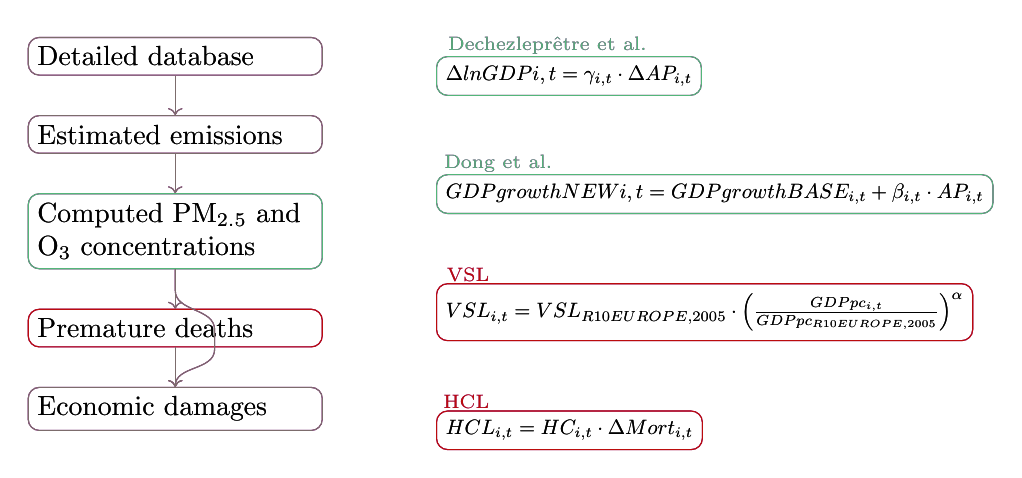
\begin{tikzpicture}[node distance = 0.5cm]
      \node[draw=mypurple,rectangle,rounded corners, text width = 3.5cm] at (-4,0) (eng) {Detailed database};
      \node[draw=mypurple,rectangle,rounded corners, text width = 3.5cm] (emi) [below = of eng] {Estimated emissions};    
      \node[draw=mypurple,rectangle,rounded corners, text width = 3.5cm] (conc) [below = of emi] {Computed \pmm\ and \oo\ concentrations};    
      \node[draw=mypurple,rectangle,rounded corners, text width = 3.5cm] (mort) [below = of conc] {Premature deaths};    
      \node[draw=mypurple,rectangle,rounded corners, text width = 3.5cm] (econ) [below = of mort] {Economic damages};  
      
      \node[draw=mypurple,rectangle,rounded corners] at (1,-0.25) (eqDech) {\scalebox{0.75}{$\Delta ln GDP{i,t} = \gamma_{i,t} \cdot \Delta AP_{i,t}$}};
      \node[draw=mypurple,rectangle,rounded corners,anchor=west] (eqDong) at ([yshift=-1.5cm]eqDech.west) {\scalebox{0.75}{${GDPgrowthNEW{i,t} = GDPgrowthBASE_{i,t} + \beta_{i,t} \cdot AP_{i,t}}$}};
      \node[draw=mypurple,rectangle,rounded corners,anchor=west] (eqVSL) at ([yshift=-1.5cm]eqDong.west) {\scalebox{0.75}{$VSL_{i,t} = VSL_{R10EUROPE,2005} \cdot \left(\frac{GDPpc_{i,t}}{GDPpc_{R10EUROPE,2005}} \right) ^ \alpha$}};
      \node[draw=mypurple,rectangle,rounded corners,anchor=west] (eqHCL) at ([yshift=-1.5cm]eqVSL.west) {\scalebox{0.75}{$HCL_{i,t} = HC_{i,t} \cdot \Delta Mort_{i,t}$}};

      \node[above left] at ([xshift=2.8cm, yshift=-0.1cm]eqDech.north west) {$\scriptstyle{\text{\textcolor{mypurple}{Dechezleprêtre et al.}}}$};
      \node[above left] at ([xshift=1.6cm, yshift=-0.1cm]eqDong.north west) {$\scriptstyle{\text{\textcolor{mypurple}{Dong et al.}}}$};
      \node[above left] at ([xshift=0.8cm, yshift=-0.1cm]eqVSL.north west) {$\scriptstyle{\text{\textcolor{mypurple}{VSL}}}$};
      \node[above left] at ([xshift=0.8cm, yshift=-0.1cm]eqHCL.north west) {$\scriptstyle{\text{\textcolor{mypurple}{HCL}}}$};

      % Arrows
      \draw [->,mypurple] (eng) to [out=270,in=90] (emi);
      \draw [->,mypurple] (emi) to [out=270,in=90] (conc);
      \draw [->,mypurple] (conc) to [out=270,in=90] (mort);
      \draw [->,mypurple] (mort) to [out=270,in=90] (econ);
      \draw [->,mypurple] (conc) to [out=270,in=90] ++(0,-0.75) to [out=270,in=90] ++(0.5,-0.5) to [out=270,in=90] ++(0,-0.25) to [out=270,in=90] (econ);

      \only<2>{       
        \node[draw=mygray,rectangle,rounded corners, text width = 3.5cm] at (-4,0) (eng) {Detailed database};
        \node[draw=mygray,rectangle,rounded corners, text width = 3.5cm] (emi) [below = of eng] {Estimated emissions};    
        \node[draw=mygreen,rectangle,rounded corners, text width = 3.5cm] (conc) [below = of emi] {Computed \pmm\ and \oo\ concentrations};    
        \node[draw=myred,rectangle,rounded corners, text width = 3.5cm] (mort) [below = of conc] {Premature deaths};    
        \node[draw=mygray,rectangle,rounded corners, text width = 3.5cm] (econ) [below = of mort] {Economic damages};  
        
        \node[draw=mygreen,rectangle,rounded corners] at (1,-0.25) (eqDech) {\scalebox{0.75}{$\Delta ln GDP{i,t} = \gamma_{i,t} \cdot \Delta AP_{i,t}$}};
        \node[draw=mygreen,rectangle,rounded corners,anchor=west] (eqDong) at ([yshift=-1.5cm]eqDech.west) {\scalebox{0.75}{${GDPgrowthNEW{i,t} = GDPgrowthBASE_{i,t} + \beta_{i,t} \cdot AP_{i,t}}$}};
        \node[draw=myred,rectangle,rounded corners,anchor=west] (eqVSL) at ([yshift=-1.5cm]eqDong.west) {\scalebox{0.75}{$VSL_{i,t} = VSL_{R10EUROPE,2005} \cdot \left(\frac{GDPpc_{i,t}}{GDPpc_{R10EUROPE,2005}} \right) ^ \alpha$}};
        \node[draw=myred,rectangle,rounded corners,anchor=west] (eqHCL) at ([yshift=-1.5cm]eqVSL.west) {\scalebox{0.75}{$HCL_{i,t} = HC_{i,t} \cdot \Delta Mort_{i,t}$}};
  
        \node[above left] at ([xshift=2.8cm, yshift=-0.1cm]eqDech.north west) {$\scriptstyle{\text{\textcolor{mygreen}{Dechezleprêtre et al.}}}$};
        \node[above left] at ([xshift=1.6cm, yshift=-0.1cm]eqDong.north west) {$\scriptstyle{\text{\textcolor{mygreen}{Dong et al.}}}$};
        \node[above left] at ([xshift=0.8cm, yshift=-0.1cm]eqVSL.north west) {$\scriptstyle{\text{\textcolor{myred}{VSL}}}$};
        \node[above left] at ([xshift=0.8cm, yshift=-0.1cm]eqHCL.north west) {$\scriptstyle{\text{\textcolor{myred}{HCL}}}$};
  
        % Arrows
        \draw [->,mygray] (eng) to [out=270,in=90] (emi);
        \draw [->,mygray] (emi) to [out=270,in=90] (conc);
        \draw [->,mygray] (conc) to [out=270,in=90] (mort);
        \draw [->,mygray] (mort) to [out=270,in=90] (econ);
        \draw [->,mygray] (conc) to [out=270,in=90] ++(0,-0.75) to [out=270,in=90] ++(0.5,-0.5) to [out=270,in=90] ++(0,-0.25) to [out=270,in=90] (econ);
      }
  \end{tikzpicture}   
\end{frame}




% %------------------------------------------------

\section{Statistical methods to analyze the results} 
\begin{frame}
\begin{center}
\Huge Four \textcolor{mygreen}{Statistical methods} to analyze the results
\end{center}
\end{frame}
%------------------------------------------------

% Sensitivity analysis ------------------------------------------------
% Looking closely at the probability density of the HCL and Dong et al. equations, we see how
% similar both shapes are. These two functions estimate the avoided damage considering the cost of mitigation, 
% which drives the result. The VSL and Dechezleprêtre
% et al. avoided damage account for the indirect impact of air pollution on GDP but
% do not account for the direct cost of mitigation. If considered, the damage through
% these equations will be much higher.
\begin{frame}
    \frametitle{Sensitivity analysis}
    \begin{figure}[htb!]
        \centering
        \includegraphics[width = \linewidth]{Images_statistical_meth/econ_uncertainty_2030.pdf}
    \end{figure}    
    \vfill \hfill \cite{rodes-bachs_beyond_ap}
\end{frame}


% Motivation: comparing climate policies ------------------------------------------------

\begin{frame}
    \frametitle{\scalebox{0.85}{Probability distribution \& Cummulative frequency graphs}}
    \begin{figure}[htb!]
        \centering
        \includegraphics[width = \linewidth]{Images_statistical_meth/econ_cobenefits_2030.pdf}
    \end{figure}    
    \vfill \hfill \tiny{\cite{rodes-bachs_beyond_ap}}
\end{frame}
\begin{frame}
    \frametitle{\scalebox{0.85}{Probability distribution \& Cummulative frequency graphs}}
    \begin{figure}[htb!]
        \centering
        \includegraphics[width = 0.8\linewidth]{Images_statistical_meth/extended_econ_cobenefits_2030.pdf}
    \end{figure}    
    \vfill \hfill \tiny{\cite{rodes-bachs_beyond_ap}}
\end{frame}



% Binomial distribution ------------------------------------------------
\begin{frame}
    \frametitle{Binomial distribution}

    \begin{figure}
        \centering
        \includegraphics[width = 0.5\linewidth]{extraFigs/binomial_eq.png}
    \end{figure}
\end{frame}
\begin{frame}
    \frametitle{Binomial distribution}

    \begin{figure}
        \centering
        \includegraphics[width = 0.30\linewidth]{extraFigs/binomial_eq.png}
        \includegraphics[width = \linewidth]{extraFigs/binomial_distrib.png}
    \end{figure}
\end{frame}

% Heavy tails ------------------------------------------------
\begin{frame}
    \frametitle{Heavy Tails}
    % There is no unique definition of a heavy-tailed distribution. Indeed, this notion only makes sense in the context of each considered model.
    % What we usually expect when we talk about heavy-tailed phenomena is some kind of different qualitative behavior of the underlying model, i.e.,
    % some deviation from the ``normal behavior'' which is caused by the extremes of the sample~\cite{Bryson1974}. Precisely because of that, 
    % heavy-tailed distributions tend to have many outliers with very high values. The heavier the tail, the larger the probability to have one 
    % or more disproportionate values in a sample; and in our case, the larger probability of high mortality outcomes.

    % Although it does not exist a universal definition, there is a general consensus and acceptance of the following one:
    \begin{alertblock}{Definition: heavy-tailed probability distribution, \cite{foss_heavy-tailed_2013}}
        A probability distribution $F(x)$ is heavy-tailed if and only if
        \begin{equation*}
            \int_\R e^{\lambda x} F(x) dx = \infty, \ \forall \lambda > 0.
        \end{equation*}    
    \end{alertblock}
    % Intuitively, a probability distribution is called heavy-tailed if it has a tail that’s
    % heavier than an exponential distribution [4]. In other words, a distribution that is
    % heavy-tailed goes to zero slower than one with exponential tails. On the contrary,
    % if a function is light-tailed, it goes to zero quicker than one with exponential tails.
    \pause{
    Intuitively:
    \begin{figure}[htb!]
        \centering
        \includegraphics[width = 0.5\linewidth]{Images_statistical_meth/Tail.png}
    \end{figure}
    }  
\end{frame}
\begin{frame}
    \frametitle{Outliers analysis}
    One way of measuring the tail heaviness is computing the \textbf{tail index} [\cite{haan_extreme_2006}]\pause, \textcolor{myred}{but you required a lot of estimates.}

    \vspace{0.5cm}
    \pause{We can relay on a finite sample argument relative to the binomial random behavior of threshold exceedances.}
\end{frame}
\begin{frame}
    \frametitle{Outliers analysis}
    Consider the sequence of economic damage for a given region and year: 
    \[ X_t^1, X_t^2, X_t^3, ..., X_t^n, \; t \in \{2020, 2030 ...\} \]
    \pause Consider a \textit{high} thereshold $h$ given by the $90^{th}$ percentile of the economic damages of that region

    \pause Consider the probability of exceeding the thereshold value $h$:
    \[ p = P(X_t^i > h) \; \forall i \in \{1,...,n\}\]
    \pause Assume that this are observations from independent random variables. Thus,
    \[ \sum_{i = 1}^n \mathbbm{1}\left( X_t^{(i)} > h\right) \sim \text{Bin}(n,p) \] 
    i.e., the number of exceedances on $n$ trials follows a binomial distribution with success probability $p$.
    % This probability provides an indication of the heaviness of
    % the tail distribution. In particular, as p increases, fatter is the distribution’s tail.
    % Although with this procedure we can not obtain a precise indication of the tail
    % heaviness, we do identify the distribution with the heavier tail, which fits exactly
    % our analysis aim
\end{frame}
\begin{frame}
    \frametitle{Outliers analysis}
    \begin{figure}[htb!]
        \centering
        \includegraphics[width = 0.6\linewidth]{Images_statistical_meth/tail_heaviness_WORLD.pdf}
    \end{figure}    
    \vfill \hfill \tiny{\cite{rodes-bachs_beyond_ap}}
\end{frame}


% Kolmogorov-Smirnov test ------------------------------------------------
\begin{frame}
    \frametitle{Kolmogorov-Smirnov test}
    % We consider the Kolmogorov-Smirnov two-sample test, which is an adaptation
    % of the non-parametric Kolmogorov-Smirnov one-sample test. It compares the
    % empirical distribution function of two samples. Intuitively, the test answers the
    % question “What is the probability that these two sets of samples were drawn from
    % the same (but unknown) probability distribution?”
    Consider two distribution functions.

    \vspace{0.5cm}
    \pause Intuitively, the test answers: ``What is the probability that these two sets of samples were drawn from
    the same (but unknown) probability distribution?''
    
    \vspace{0.5cm}
    \pause
    In a more formal way:
    \[
    \left\{\begin{array}{ll}
        H_0: & F_X(x) = F_Y(x) \ \  \forall x, \\
        H_1: & F_X(x) \neq F_Y(x) \ \ \text{for some }x
    \end{array}\right.
    \]
    \pause
    which is equivalent to
    \[
    \left\{\begin{array}{ll}
        H_0: & \scalebox{0.95}{\text{NZ and EoC climate policies have the \textbf{same} distribution function},} \\
        H_1: & \scalebox{0.95}{\text{NZ and EoC climate policies have the \textbf{different} distribution function}}
    \end{array}\right.
    \]
\end{frame}

\begin{frame}
    \frametitle{Kolmogorov-Smirnov test}
    \begin{figure}[htb!]
        \centering
        \includegraphics[width = 0.98\linewidth]{Images_statistical_meth/ks_econ_2030_2050.pdf}
    \end{figure}    
    \vfill \hfill \tiny{\cite{rodes-bachs_beyond_ap}}
\end{frame}


% %------------------------------------------------

\section{Summary \& Discussion} 
\begin{frame}
  \frametitle{Summary \& Discussion}
  \begin{itemize}
      \setlength\itemsep{1em}
      \pause \item Does \emph{net-zero} climate policy have significantly more co-benefits for air pollution damages outcomes?
      \pause \item Does \emph{net-zero} climate policy increase the economic co-benefits?
      \pause \item What contributes more to the uncertainty in air pollution economic outcomes: emissions uncertainty, impact functions uncertainty, econometric equations, or the elasticity choice?
      \pause \item How does the \emph{net-zero} climate policy affect the tails' heaviness?
      \pause \item Which regions will benefit the most from the \emph{net-zero} climate policy? And when will these benefits be more tangible, in the near term or in the mid-century?
  \end{itemize}
\end{frame}
  
% %------------------------------------------------

\section{Master Thesis Proposal} 
\begin{frame}
\begin{center}
\Huge Master Thesis Proposal
\end{center}
\end{frame}
%------------------------------------------------
    
\begin{frame}
    \frametitle{Health impacts of \pmm\ \& \oo}
    \centering
    \href{https://vizhub.healthdata.org/gbd-compare/}{\textcolor{blue}{IHME database}}
    \href{https://vizhub.healthdata.org/gbd-compare/}{(\textcolor{blue}{\texttt{https://vizhub.healthdata.org/gbd-compare/}})}
\end{frame}

\begin{frame}
\frametitle{Analysis of \textcolor{mygreen}{health impacts} attributable to \textcolor{mypurple}{household}  \textcolor{white}{......}  \textcolor{mypurple}{air pollution} associated with alternative futures}
The \textbf{objective} of this internship is to develop an \textbf{econometric model} to \textcolor{mygreen}{calculate future household air pollution and its subsequent impacts}.

\onslide<2->{It will be \textcolor{mygreen}{incorporated into a well-reputed integrated assessment model} (GCAM) 
and the econometric model developed during the internship will be written as a \textbf{standalone R-package} and is \textcolor{mygreen}{planned to be published} at JOSS.}

\onslide<3->{\textcolor{mypurple}{Methodology}: Panel data analysis \& econometrics}

\onslide<4->{\textcolor{mypurple}{Prerequisites}: 
\begin{itemize}
    \item Advanced experience in econometrics and econometric-software (ideally R) 
    \item Panel data analysis
    \item Data processing, curation, and visualization (large databases)
    \item Spanish knowledge    
\end{itemize}
}

\onslide<5->{If you are interested, see the full proposal \href{https://github.com/klau506/lecture_AP_damage/blob/main/Proposal_TFM_BC3_HAP.pdf}{\textcolor{blue}{here}} and write at \textcolor{blue}{\texttt{jon.sampedro@bc3research.org}}
 and \textcolor{blue}{\texttt{inaki.arto@bc3research.org}}
\begin{tikzpicture}[remember picture,overlay]
    \node[draw=white,rectangle,rounded corners] at (-0.5,1) (QR) {\includegraphics[width=1.25cm]{"extraFigs/TFM_QR.png"}};
\end{tikzpicture}
}

\end{frame}

% %------------------------------------------------

\begin{frame}
\centering
    Thank you for your attention!!\\
    \vspace{1cm}
    Questions?\\
    \vspace{3cm}
    \small\textcolor{mygreen}{claudia.rodes@bc3research.org}
\end{frame}

%------------------------------------------------

\addtocounter{framenumber}{-1}
\begin{frame}[allowframebreaks]
\frametitle{Bibliography}
\bibliographystyle{apalike}
\bibliography{myLibrary}
\end{frame}

%------------------------------------------------

% \section{Extra Slides} 
\begin{frame}
\begin{center}
\Huge Extra Slides
\end{center}
\end{frame}
%---------------------

% \subsection{Pollutants and health impacts}
\begin{frame}
\frametitle{Pollutants main precursors}
\centering
    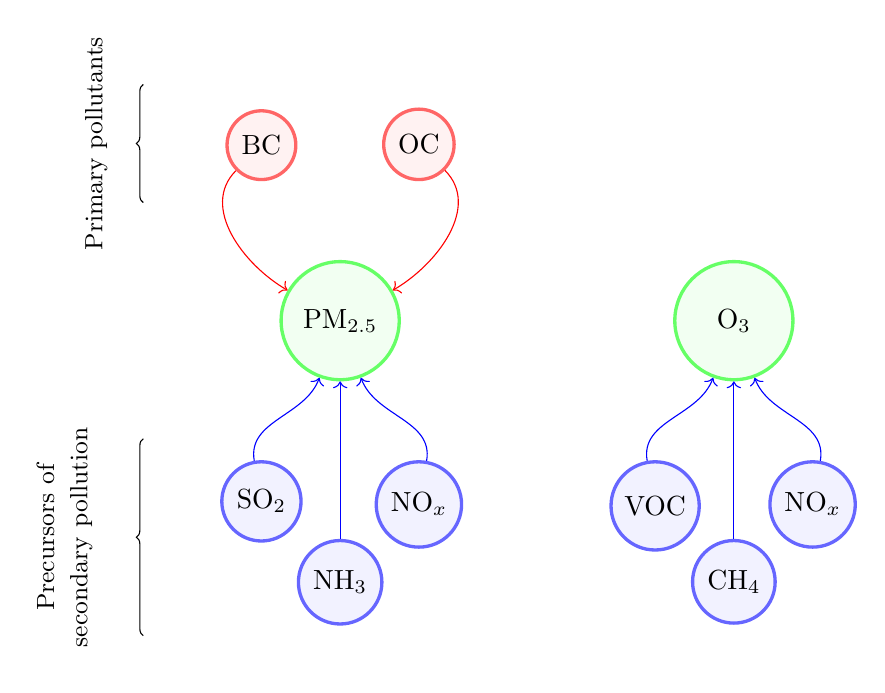
\begin{tikzpicture}[
    roundnode1/.style={circle, draw=green!60, fill=green!5, very thick, minimum size=15mm},
    roundnodeP/.style={circle, draw=red!60, fill=red!5, very thick, minimum size=5mm},
    roundnodeS/.style={circle, draw=blue!60, fill=blue!5, very thick, minimum size=5mm},
    ]
    %Nodes
    \node[roundnode1]   (pmm)         at (2,0) {\pmm};
    \node[roundnodeP]   (pmmBC)       [above=of pmm, xshift=-1cm] {BC};
    \node[roundnodeP]   (pmmOC)       [above=of pmm, xshift=1cm] {OC};
    \node[roundnodeS]   (pmmSO2)      [below=of pmm, xshift=-1cm] {SO$_2$};
    \node[roundnodeS]   (pmmNOx)      [below=of pmm, xshift=1cm] {NO$_x$};
    \node[roundnodeS]   (pmmNH3)      [below=of pmm, yshift=-1cm] {NH$_3$};
    \node[roundnode1]   (oo)         at (7,0) {\oo};
    \node[roundnodeS]   (ooVOC)      [below=of oo, xshift=-1cm] {VOC};
    \node[roundnodeS]   (ooNOx)      [below=of oo, xshift=1cm] {NO$_x$};
    \node[roundnodeS]   (ooCH4)      [below=of oo, yshift=-1cm] {CH$_4$};
    
    %Lines
    \draw [->,red]  (pmmBC) to [out=225,in=150] (pmm);
    \draw [->,red]  (pmmOC) to [out=315,in=30] (pmm);
    \draw [->,blue] (pmmSO2) to [out=100,in=250] (pmm);
    \draw [->,blue] (pmmNOx) to [out=80,in=290] (pmm);
    \draw [->,blue] (pmmNH3) -- (pmm);
    \draw [->,blue] (ooVOC) to [out=100,in=250] (oo);
    \draw [->,blue] (ooNOx) to [out=80,in=290] (oo);
    \draw [->,blue] (ooCH4) -- (oo);

    % Simple brace
    \draw [decorate, decoration = {brace,mirror}] (-0.5,3) --  (-0.5,1.5) node [black,midway,xshift=-0.6cm,rotate = 90] {\small{Primary pollutants}};
    \draw [decorate, decoration = {brace}] (-0.5,-4) --  (-0.5,-1.5) node [black,midway,xshift=-1cm,rotate=90,text width=3cm,align=center] {\small{Precursors of secondary pollution}};
    \end{tikzpicture}
\end{frame}

\begin{frame}{Health impacts (mortality) equations}
\begin{center}
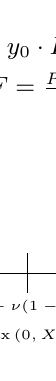
\begin{tikzpicture}[trim left=(concExtra), trim right = (concExtra), node distance = 0.15cm]
    \node (concExtra) at (0,0) {};

    % Equations MORTALITY
    \node (PD1) [below of=concExtra,yshift=0cm,align=center]{\small{$\Delta Mort = y_0 \cdot PAF \cdot pop$}};;
    \node (PAF) [below of=concExtra,yshift=-0.5cm,align=center]{\small{$ PAF = \frac{RR-1}{RR}$}};;

    % timeline    
    \node (LL) [below of=concExtra,xshift=-3cm,yshift=-2.35cm,align=center]{\tiny{$LL(X) = \exp\{\beta(X-X_0)\}$}};;
    \node (IER1) [below of=concExtra,xshift=0cm,yshift=-3.25cm,align=center]{\tiny{$IER(X) = 1-\nu (1-\exp\{-\omega z^\delta\}),$}};;
    \node (IER2) [below of=IER1,align=center,yshift=-0.25cm]{\tiny{$z = \max{(0,X-X_0)}$}};;
    \node (GEMM1) [below of=concExtra,xshift=2.5cm,xshift=1.5cm,yshift=-1.75cm,align=center]{\tiny{$GEMM(X) = \exp\left\{\frac{\theta \log\left(\frac{z}{\alpha+1}\right)}{1+\exp\{-\frac{z-\mu}{\nu}\}}\right\},$}};;
    \node (GEMM2) [below of=GEMM1,align=center,yshift=-0.43cm]{\tiny{$z = X - \min{(X)}$}};;
    
    \node (time) [below of=concExtra,align=center,xshift=5.5cm,yshift=-2.75cm]{\tiny{time}};;
    \draw[->] (-6,-3) -- (6,-3); 
    \draw (-3,-2.75) -- (-3,-3.25);
    \draw (0,-2.75) -- (0,-3.25);
    \draw (4,-2.75) -- (4,-3.25);
\end{tikzpicture}
\end{center}
\end{frame}

\begin{frame}{Health impacts uncertinaty}
\begin{figure}
    \centering
    \includegraphics[width = \linewidth]{extraFigs/heatlh_uncertainty_2030.pdf}
\end{figure}
\vfill \hfill \tiny{\cite{rodes-bachs_beyond_ap}}
\end{frame}

\begin{frame}{Health impacts Kolmogorov-Smirnov test}
\begin{figure}
    \centering
    \includegraphics[width = 0.98\linewidth]{extraFigs/ks_mort_2030_2050.pdf}
\end{figure}
\vfill \hfill \tiny{\cite{rodes-bachs_beyond_ap}}
\end{frame}


% GCAM slides --------------------------------------------------------------------------------------

\begin{frame}{GCAM}
    The Global Change Analysis Model (GCAM) in a figure:
\begin{figure}
    \centering
    \includegraphics[width = 0.5\linewidth]{extraFigs/GCAM_diagram_basic.jpg}
\end{figure}
\vfill\hfill \tiny{Source: \url{https://github.com/JGCRI/gcam-doc}}
\end{frame}

\begin{frame}{GCAM}
\begin{itemize}  \setlength\itemsep{5pt}
    \item The Global Change Analysis Model (GCAM) is an open-source community model developed by Joint Global Change Research Institute (JGCRI) (University of Maryland, MA, USA)
    \item It is a partial-equilibrium, multisector, integrated assessment model designed to explore human and Earth-system dynamics
    \item GCAM analyses the interdependencies between global energy, AFOLU, water, emissions, and climate systems within a single computational platform from now to 2100
    \item The model has been widely used for IPCC scenarios, SSP pathways, and several multisector multiscale studies and reports
\end{itemize}
\end{frame}

\begin{frame}{GCAM evolution}
\begin{figure}
    \centering
    \includegraphics[width = 0.95\linewidth]{extraFigs/GCAM_evolution.jpg}
\end{figure}
\vfill\hfill \tiny{Source: \url{https://github.com/JGCRI/gcam-doc}}
\end{frame}

\begin{frame}{GCAM inputs and outputs}
\begin{figure}
    \centering
    \includegraphics[width = 0.95\linewidth]{extraFigs/GCAM_input_output.png}
\end{figure}
\vfill\hfill \footnotesize{Source: \url{https://github.com/JGCRI/gcam-doc}}
\end{frame}

\begin{frame}{GCAM temporal scale and strucutre}
\begin{figure}
    \centering
    \includegraphics[width = 0.95\linewidth]{extraFigs/GCAM_temporal_structure.jpg}
\end{figure}
\vfill\hfill \tiny{Source: \url{https://github.com/JGCRI/gcam-doc}}
\end{frame}

\begin{frame}{GCAM spatial layers}
    \begin{itemize}
        \item The core version of GCAM divides the entire World in 32 geopolitical regions and 235 water basins
        \item The land regions (384) are the intersection between regions and water basins
        \item There is a single global region for climate system impacts
    \end{itemize}
    \begin{figure}
        \centering
        \includegraphics[width = 0.8\linewidth]{extraFigs/GCAM_spatial_layers.jpg}
    \end{figure}
    \vfill\hfill \tiny{Source: \url{https://github.com/JGCRI/gcam-doc}}
\end{frame}

\begin{frame}{GCAM prices, competition, and funcional forms}
    \begin{columns}[T] 
        \begin{column}{0.48\textwidth} 
            \centering
            \includegraphics[width=\textwidth]{extraFigs/GCAM_prob_approach.png}
        \end{column}
        \begin{column}{0.48\textwidth}
            \begin{itemize} \setlength\itemsep{5pt}
                \item Calibrated logit approach assumes a distribution of realized costs due to heterogeneous conditions
                \item Market share based on probability that a technology has the least cost for an application, avoiding a ``winner take all'' result
                \item Historical calibration influences future competition through the ``share-weight''
            \end{itemize}
        \end{column}
    \end{columns}
    \vfill\hfill \tiny{Source: \url{https://github.com/JGCRI/gcam-doc}}
\end{frame}

\begin{frame}{GCAM ecosystem}
    \begin{figure}
        \centering
        \includegraphics[width = 0.8\linewidth]{extraFigs/GCAM_diagram.jpg}
    \end{figure}
    \vfill\hfill \tiny{Source: \url{https://github.com/JGCRI/gcam-doc}}
\end{frame}
    
% GCAM systems -----------------------------------------------------------------
\begin{frame}{GCAM Energy system}
    \begin{columns}[T] 
        \begin{column}{0.60\textwidth} 
            \centering
            \includegraphics[width=0.6\textwidth]{extraFigs/GCAM_energy_system_breakout.png}
            \includegraphics[width=\textwidth]{extraFigs/GCAM_energy_system.png}
            \vfill\hfill \tiny{Source: \url{https://github.com/JGCRI/gcam-doc}}
        \end{column}
        \begin{column}{0.38\textwidth}
            \begin{itemize}
                \item Regional Energy production, transformation, and end-use demand are based on economic functions of resources, technologies, prices, population, and income
                \item Energy transformation and end-use consumption are represented by specific, bottom-up technologies in most sectors
            \end{itemize}
        \end{column}
    \end{columns}
\end{frame}

\begin{frame}{GCAM Land system}
    \begin{columns}[T] 
        \begin{column}{0.54\textwidth} 
            \centering
            \includegraphics[width=0.6\textwidth]{extraFigs/GCAM_land_system_breakout.png}
            \includegraphics[width=\textwidth]{extraFigs/GCAM_land_system.png}
            \vfill\hfill \tiny{Source: \url{https://github.com/JGCRI/gcam-doc}}
        \end{column}
        \begin{column}{0.45\textwidth}
            \begin{itemize}
                \item All land cover and use, including all commercial land uses as well as non-commercial natural lands, are represented in GCAM
                \item These land categories are represented in each of the 384 land regions (where applicable) and calibrated to match a historical base year
                \item Economics drive future changes in cropland, pasture, forest, and other land uses
            \end{itemize}
        \end{column}
    \end{columns}
\end{frame}
    
\begin{frame}{GCAM Water system}
    \begin{columns}[T] 
        \begin{column}{0.60\textwidth} 
            \centering             
            \includegraphics[width=0.6\textwidth]{extraFigs/GCAM_water_system_breakout.png}
            \includegraphics[width=0.85\textwidth]{extraFigs/GCAM_water_system.png}
            \vfill\hfill \tiny{Source: \url{https://github.com/JGCRI/gcam-doc}}
        \end{column}
        \begin{column}{0.38\textwidth}
            \begin{itemize}
                \item Runoff from Xanthos model with global climate data 
                \item Non-renewable groundwater/depletable resource curves 
                \item Water supply and demand are economically-balanced in each river basin
            \end{itemize}
        \end{column}
    \end{columns}
\end{frame}
    
\begin{frame}{GCAM Climate system}
    \begin{columns}[T] 
        \begin{column}{0.51\textwidth} 
            \centering     
            \includegraphics[width=0.6\textwidth]{extraFigs/GCAM_climate_system_breakout.png}
            \includegraphics[width=\textwidth]{extraFigs/GCAM_climate_system.png}
            \vfill\hfill \tiny{Source: \url{https://github.com/JGCRI/gcam-doc}}
        \end{column}
        \begin{column}{0.48\textwidth}
            \begin{itemize}
                \item GCAM passes emissions to Hector:
                \begin{multicols}{2}
                    \begin{itemize}
                        \item Fossil $CO_2$ (FA)
                        \item Land-Use $CO_2$ (FLC)
                        \item $CH_4$
                        \item $N_2O$
                        \item 26 halocarbons
                        \item Pollutants: $SO_2$, $CO$, $NO_x$, $NMVOC$s, $BC$, $OC$                    
                    \end{itemize}
                \end{multicols}
                \item Hector computes atmospheric $CO_2$ concentrations, radiative forcing (direct and indirect), temperature change, air- land/sea fluxes, ocean heat flux
            \end{itemize}
        \end{column}
    \end{columns}
\end{frame}
    
% Idea: crear codi d'R i dades per a jugar amb les elasticitats i veure com afecta a cada regió

%------------------------------------------------

\end{document}